\documentclass[10pt,a4paper,twocolumn]{article}
\usepackage[utf8]{inputenc}
\usepackage[T1]{fontenc}
\usepackage{amsmath}
\usepackage{amsfonts}
\usepackage{amssymb}
\usepackage{graphicx}
\usepackage[font=small, labelfont=bf]{caption}
\graphicspath{{images/}}
\usepackage[margin=0.6in]{geometry}
\usepackage{hyperref}
\hypersetup{
	colorlinks=true,
	linkcolor=blue,
	urlcolor=blue
}



% approx (8.5 - 2*margin)/2
\newcommand\colwidth{3.5in}
\newcommand\colline{\noindent\rule{\colwidth}{2.5pt}\\}

\newcommand\bemph[1]{\textbf{\emph{#1}}}

\newcommand\imgscale{0.4}
\newcommand\optionplot[2][\imgscale]{
	\begin{center}
		\includegraphics[scale=#1]{#2}
	\end{center}
}
\newcommand\strategy[1]{{\centering\vspace{0.1in}\subsection*{ --------- #1 ---------}}}


\title{Options: Strategies and Theory}
\author{George Willingham}
\date{}

\begin{document}
	\maketitle
	
	
	\section*{Basics}
	Options are derivative securities --- tradable assets which derive their value from an underlying security. As derivatives, options offer a way to take a stake in their underlying (most often a stock) without actually owning it. Also, they offer a way to leverage a small initial investment into a larger stake. They are useful tools in trading for hedging bets and making more nuanced bets than simple bull or bear positions. The precise definition of an (American) option is the following.
	\\
	\colline
	\emph{\textbf{Options} are contracts which grant the buyer the right, but not the obligation, to buy or sell an underlying security at a specified  price up to or before a specified expiration date.}
	\colline
	So options contracts are specified by three values: the \bemph{strike price} $k$, the expiration date, and also the premium $p$ (i.e. price of the contract). Option premiums depend on many factors including the price of the underlying, the volatility of the underlying, the time to expiration, and other measures of \emph{sensitivity}. Many of these factors are quantified by a few values known as the greeks. These will be discussed later as they are an important tool for options traders.
	
   \strategy{Calls}
	A \bemph{call option} gives the buyer the right to \emph{buy} the underlying stock at the agreed upon strike price. So if the stock's value exceeds the strike price, then the owner of the call can effectively buy shares at a discount. Clearly then, a call on its own is a bullish position. So with premium $p$, strike price $k$, and underlying stock valued at $s$, a call will have payout per share given by 
	$$ \pi_\text{call}=\max(s - k, 0) - p $$
	Once the stock reaches the strike price, the payout begins to grow linearly. Since the premium was paid upfront for the option, the break-even stock value is $s_\text{be}=k+p$. This linear region (where $s>k$ for a call) is known as being \bemph{in-the-money} (ITM). The flat region of the payout curve ($s<k$) is called \bemph{out-of-the-money} (OTM) and naturally $s=k$ is called \bemph{at-the-money} (ATM).
	
	\optionplot{call.png}
	
	\strategy{Puts}
	A \bemph{put option} give the buyer the right to \emph{sell} the underlying stock at the agreed upon strike price. So if the stock's value falls below the strike price, the owner of the put has locked in a price for the stock which is higher than its value, thus making a clear profit. A put then has a bearish outlook and has payout given by 
	$$ \pi_\text{put} = \max(k - s, 0) - p $$ 
	where again $s$ is the underlying stock value, $k$ is the strike price, and $p$ is the option premium. The break-even point is $s_\text{be}=k-p$. A put is ITM when $s<k$, OTM when $s>k$, and ATM when $s=k$.
	\optionplot{put.png}
	
	\strategy{Buying vs Selling}
	Buying calls and puts always is always risk-limited since there is an upper bound on how much can be lost in the trade. On the other hand, selling options without further hedging has considerable risk. The payout for a sold call is $-\pi_\text{call}$ and similarly a sold put has payout $-\pi_\text{put}$. Selling an option brings in a nice premium and as long as the option stays OTM, it is kept as a profit on the trade. But once the underlying goes ITM, the owner of the option could exercise, obligating the seller to buy or sell the underlying shares. Large price swings can then lead to potentially catastrophic losses so it is important to only sell options with a solid understanding of the risk. Most of the time, traders do not sell naked calls or puts but instead hedge in some way to limit risk.
	
	It is important to keep in mind that a trader with an open position in an options contract has essentially two ways forward. As expiry gets closer, an option owner can either do nothing, letting the option expire, or they can \bemph{sell to close}. That is, they can sell the option away and take as payout the difference between the current premium and the premium paid to open the position. This is in fact what most options traders do. Similarly, an option seller can \bemph{buy to close} by buying back their contract and removing any obligation to the option owner. 
	\\
	
	\section*{Multi-Leg Strategies}
	Options are powerful tools that provide a way for traders to leverage a relatively small investment into a much larger stake. Using just calls and puts, it is possible to make consistent money --- specially if equity positions are combined into the full portfolio. However with single calls and puts, the basic bet remains simply either bearish or bullish. When multiple options are combined, a variety of other bets can be made and more nuanced strategies can be implemented. In particular, multi-option (multi-leg) strategies can be used to bet on volatility and stationarity. 

	\strategy{Volatility Spreads}
	The simplest two-option strategy is the \bemph{straddle}. This strategy consists of buying both a call and a put for the same stock at the same strike price and date of expiry. The resulting payout $\pi_\text{straddle} = \pi_\text{call} + \pi_\text{put}$ can be written as
	$$ \pi_\text{straddle} = |s-k| - \text{premiums} $$
	From here it is clear that a net profit is made whenever the stock value $s$ is sufficiently far away from the strike price in either direction. Specifically, the break-even points are $s_\text{be}=k\pm \text{premiums}$. So a straddle is a bet on volatility.
	\optionplot{straddle.png}
	When the call and put have different strike prices, this strategy is called either a \bemph{strangle} or a \bemph{gut spread}. In a strangle strategy, both options are bought OTM (this implies $k_\text{call} > k_\text{put}$). As a consequence the premiums paid in a strangle position are less than for a straddle. 

	In the region between strike prices, the payout is at its minimum and is constant at just the total cost of premiums. Also, the break-even points are given by $s_\text{be}=k_\text{call} + \text{premiums}$ and $s_\text{be}=k_\text{put} - \text{premiums}$. So compared with a straddle, the price swing needed to turn a profit is larger. In summary, strangles are like straddles but with lower overall downside and less probable upside.
	\optionplot{strangle.png}
	For a \emph{gut spread}, the call and put are bought ITM instead of OTM. As a consequence, the premiums are higher.
	
	\strategy{Bullish Spreads}
	Bullish spreads consist of buying one option and selling another option of the same type (call/put) but with a higher strike price. This strategy is a way of taking a bullish position while reducing risk compared to a single call. Of course, this comes with the downside that max profit is limited. Bullish spreads are either bull call or bull put spreads.
	
	A bull call spread is an options strategy with a bullish outlook consisting of buying one call that is ITM and selling another call that is OTM. The ITM call will certainly be more valuable so when entering this position there is a net debit to the trader's account. For this reason, this strategy is also called a call debit spread.
	
	\optionplot{debit_call_spread.png}
	This strategy is risk-limited but also profit-limited. The benefit over a standard call is that it is cheaper to enter this position. Also since most likely, the stock is not going to move a great deal higher than the strike price, the upper-limit on the profit is unlikely to be an issue.
	
	Alternatively, a similar position can be made with puts. A \emph{bull put spread} strategy consists of buying one OTM put and selling an ITM put for the same underlying and expiry. The ITM put will of course be more valuable so entering this position leads to a net credit at the start.
	
	\optionplot{credit_put_spread.png}
	
	\strategy{Bearish Spreads}
	Similar to the bullish vertical spreads (i.e. the bull call spread and bull put spread), we can construct bearish spreads. For this strategy, one option is bought and another of the same type is sold at a lower strike price. 
	
	With call options, one can enter a \bemph{bear call spread} by buying one OTM call and selling one ITM call. Since the ITM option will have a higher premium, a net credit is received when entering this position. For this reason, this is sometimes called a bear credit spread.
	
	\optionplot{credit_call_spread.png}
	
	\optionplot{debit_put_spread.png}
	
	\strategy{Stationary Spreads}
	

	\optionplot{butterfly_spread.png}		

	\optionplot{iron_condor.png}
	\newpage
	\section*{Stochastic Modeling of Options}
	
	\strategy{Black-Scholes Model}
	The Black-Scholes model (a.k.a the Black-Scholes-Merton or BMS model) for options pricing is one of the most famous mathematical models in finance. It won its creators a Nobel prize in economics and is still widely used today. However its shortcomings are also very well known and will be discussed. Generally speaking, the Black-Scholes equation provides a necessary condition for the price of any derivative security in an arbitrage-free market. It is most famous for its application to European options (options which cannot be exercised until expiry), but its role in the analysis of all derivatives pricing makes it worth exploring in detail.
	
	The model begins by assuming that the underlying stock evolves in time via a geometric Brownian motion process. In other words, the returns are assumed to be lognormally distributed. Formally, the stock price $s(t)$ evolves via the SDE
	$$ds(t) = \mu s(t) dt + \sigma s(t) dw(t)$$
	where $\mu$ and $\sigma$ are constant drift and volatility parameters and $w(t)$ is a standard Wiener process (Brownian motion). A call option (or any derivative with underlying $s$) will have a price which depends explicitly on both the stock value $s$ and the time $t$: $p=p(s, t)$. By It\^{o}'s lemma\footnote{It\^{o}'s lemma basically says that a Wiener process has $dw^2=dt$. So in the variation $dp = \frac{\partial p}{\partial t}dt + \frac{\partial p}{\partial s} ds + \frac{1}{2}\frac{\partial^2p}{\partial s^2}ds^2 + \dots$, the $ds^2$ term leads to an additional $dt$ term.}, we can then write a stochastic equation for the price of the option:
	$$ dp(s,t) = \left(\mu s \frac{\partial p}{\partial s} + \frac{\partial p}{\partial t} + \frac{1}{2}\sigma^2 s^2 \frac{\partial^2 p}{\partial s^2}\right)dt + \sigma s\frac{\partial p}{\partial s} dw $$
	To find a closed-form and deterministic expression for the value $p$, we will \emph{replicate} the option's value with an equivalent and simple portfolio. In particular, we consider a \emph{self-financing} portfolio consisting of a cash account $x$ growing with risk-free interest as $x(t)e^{rt}$ and some shares of the stock $s$. If $n$ denotes the number of shares of $s$, then the portfolio's value $v$ is given by
	$$ v(s,t) = n(t)s(t) + x(t)e^{rt} $$
	The goal is to find $n(t)$ and $x(t)$ such that $v$ is exactly $p$. Since it is self-financing, $v$ is independent of changes in $n$ or $x$ so  it satisfies $dv = nds + x d(e^{rt})$ or after plugging in for $ds$:
	$$ dv(s,t) = \left(\mu s n + x r e^{rt}\right)dt + \sigma s n\; dw $$
	Now comparing this with the previous expression for $dp(s,t)$, we can make $dv=dp$ by identifying terms
	\begin{align*}
		n(t)&\equiv \frac{\partial p}{\partial s} \\
		 x r e^{rt} &\equiv \frac{\partial p}{\partial t} + \frac{1}{2}\sigma^2 s^2 \frac{\partial^2 p}{\partial s^2}
	\end{align*}
	So as long as the replicating portfolio matches the option price initially, the dynamics match so we can identify $p\equiv v$ for all time. Then using the above equations, we can replace the equation for $v$ with an equation for $p$. The result is the \bemph{Black-Scholes equation} and in its conventional form, it is written:
	$$  rs\frac{\partial p}{\partial s} + \frac{\partial p}{\partial t} + \frac{1}{2}\sigma^2 s^2 \frac{\partial^2 p}{\partial s^2} - r p = 0 $$
	So now the PDE must be solved to obtain $p$, but to do so, boundary conditions must be established. This is a "backwards" parabolic PDE so for a unique solution we need a \emph{final} condition rather than an initial condition. For the call option, we choose the final condition at expiration time $T$: $ p(s, T) = \max(s - k, 0) $ where $k$ is the call strike price. The stock value is defined on $s\in[0,\infty)$ so we need boundary conditions at zero and infinity. We make the choices: $p(0, t) = 0$ and $p(s,t)\to s - ke^{-r(T-t)}$ as $s\to\infty$. With these conditions, the solution to the Black-Scholes equation can be found. Defining the time until expiry as $\tau\equiv T - t$, we can nicely write the solution, known as the \bemph{Black-Scholes formula}:
	
	$$ p_\text{call}(s,\tau) = s\Phi\left(d_+\right)  - e^{-r\tau} k \Phi\left(d_-\right) $$
	\begin{figure}[t!]
	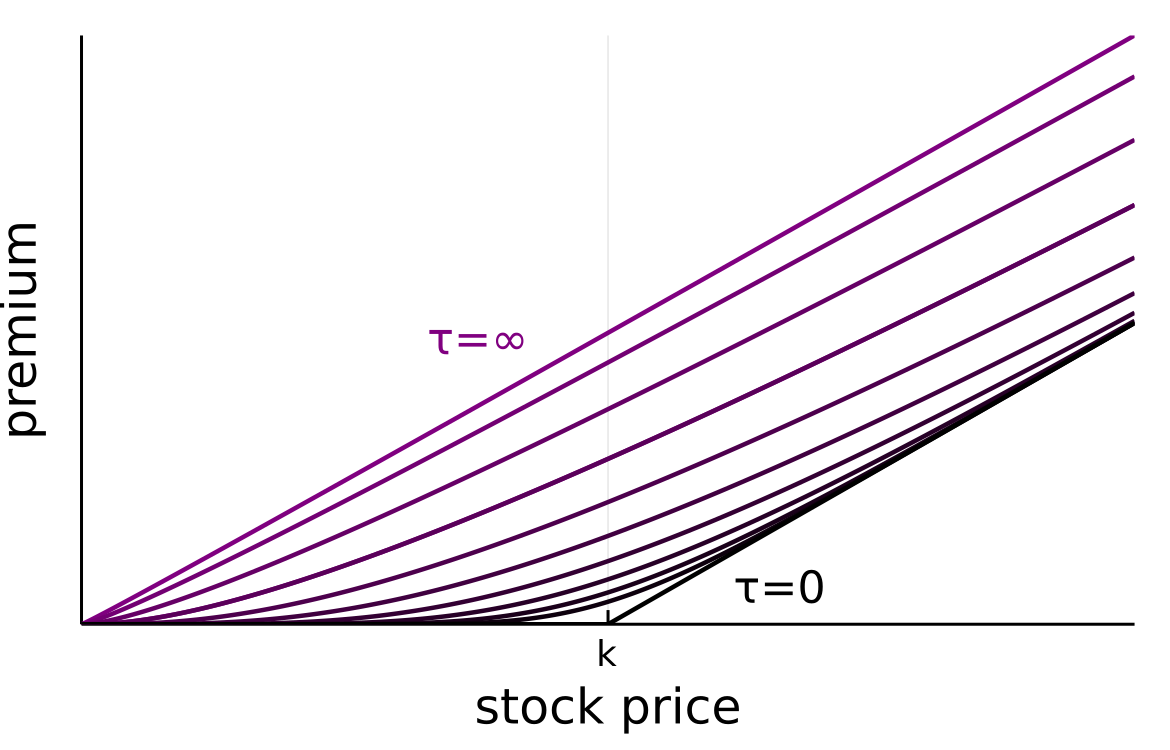
\includegraphics[scale=0.2]{black_scholes_prices.png}
	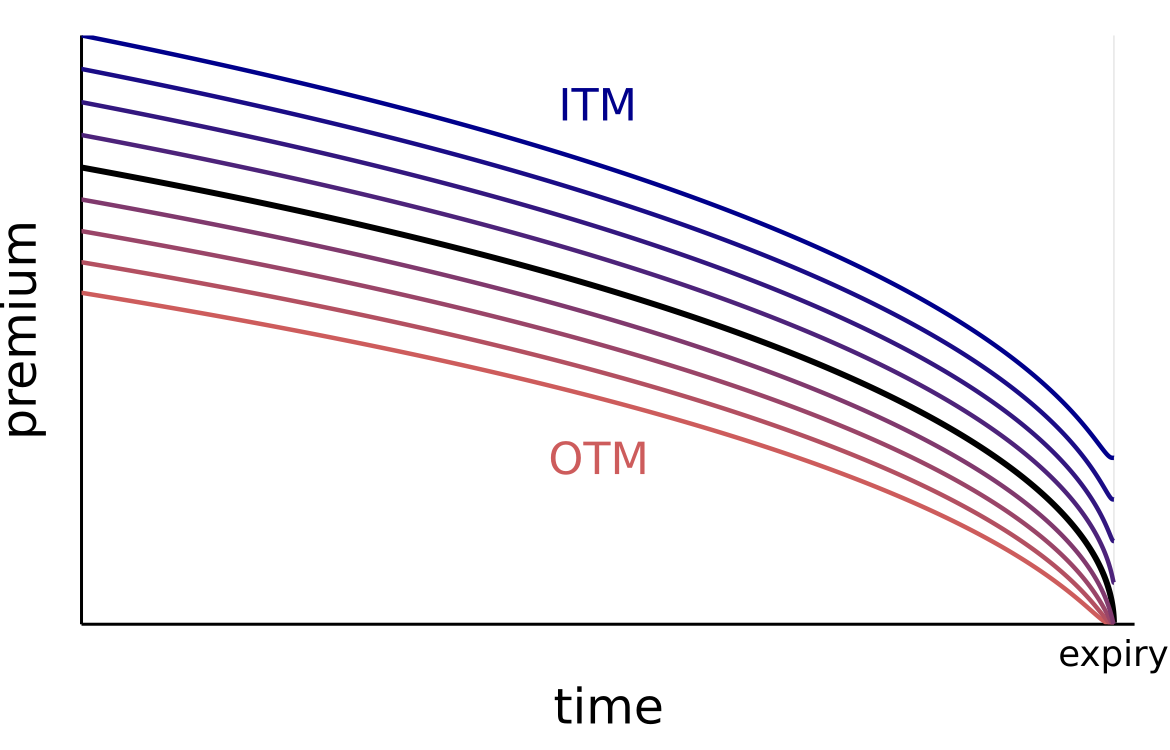
\includegraphics[scale=0.2]{theta_decay.png}
	\caption{Black-Scholes formula for European call pricing}
	\end{figure}
	\begin{figure*}[ht]
	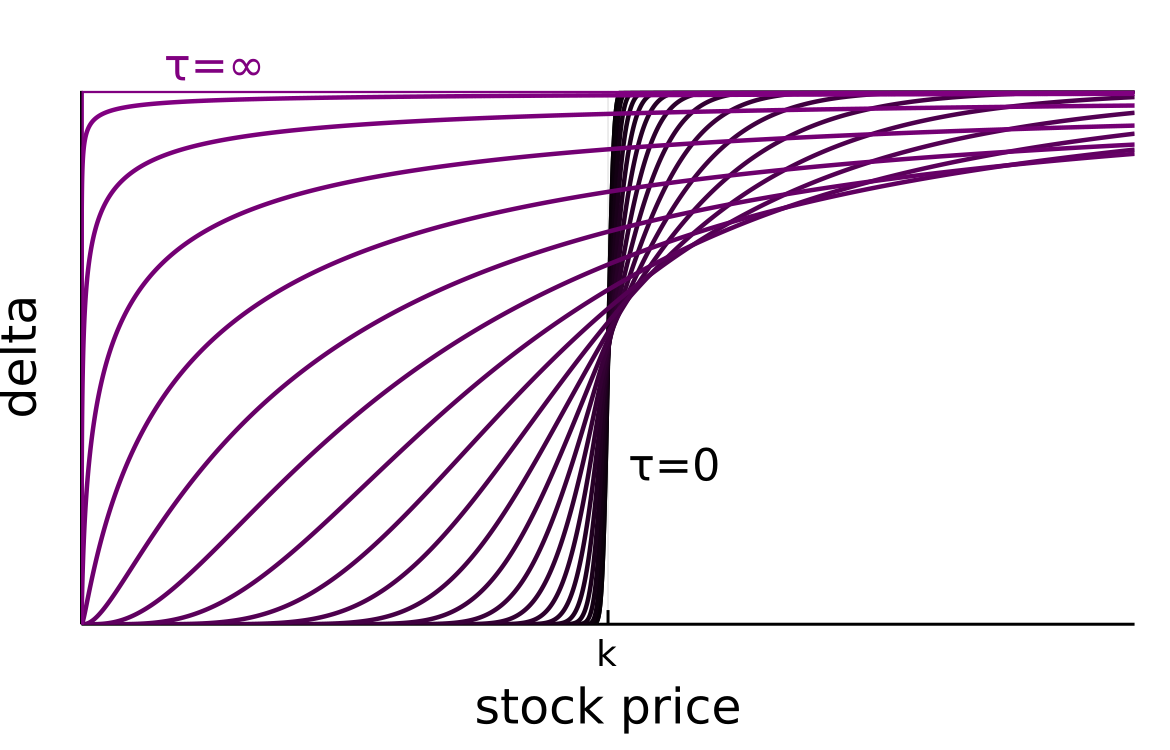
\includegraphics[scale=0.145]{delta.png}
	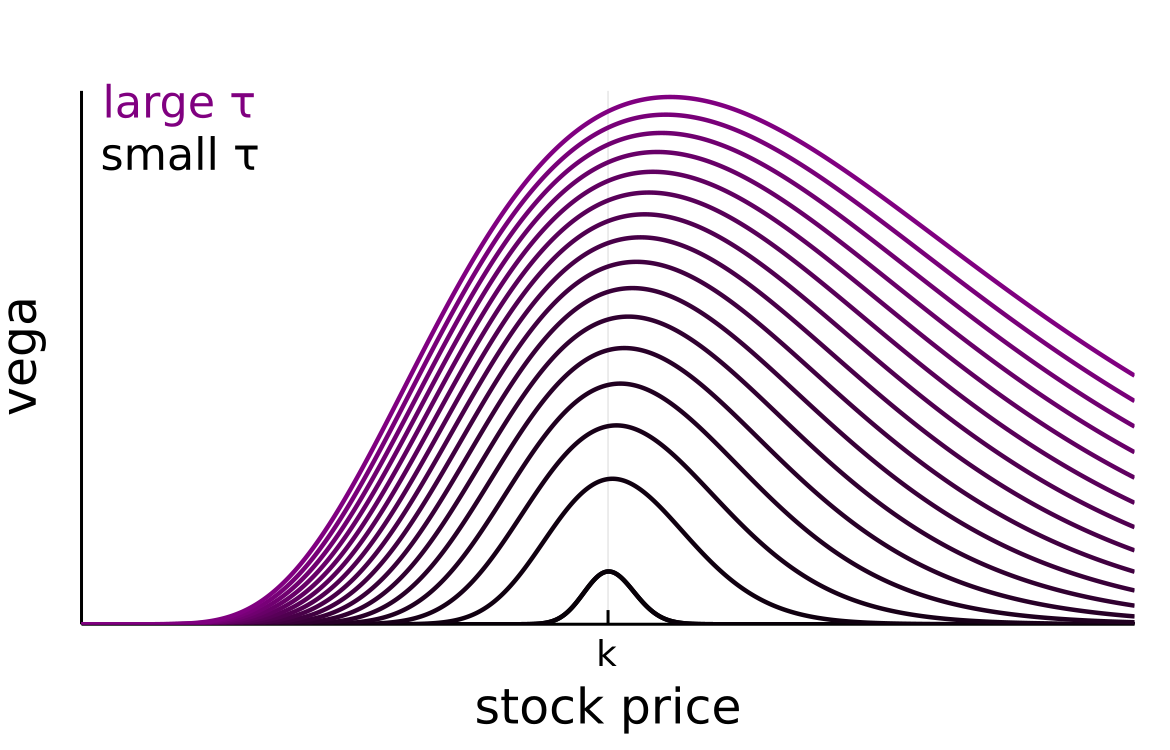
\includegraphics[scale=0.145]{vega.png}
	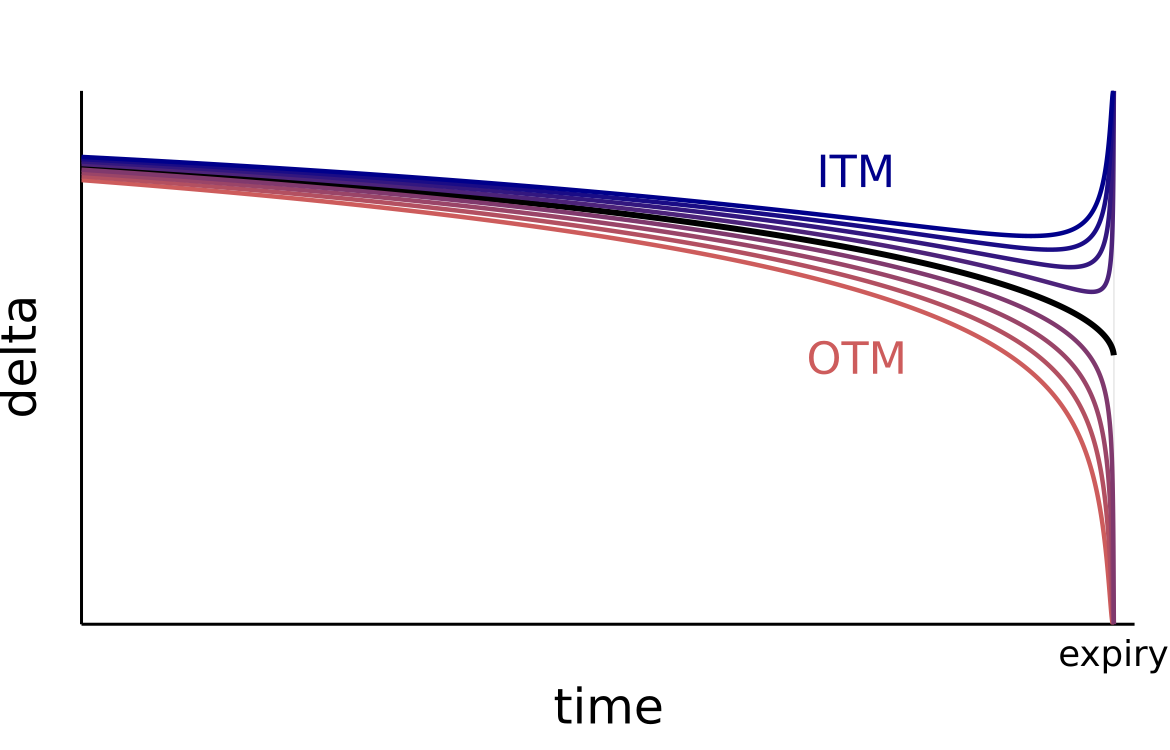
\includegraphics[scale=0.145]{delta_time.png}
	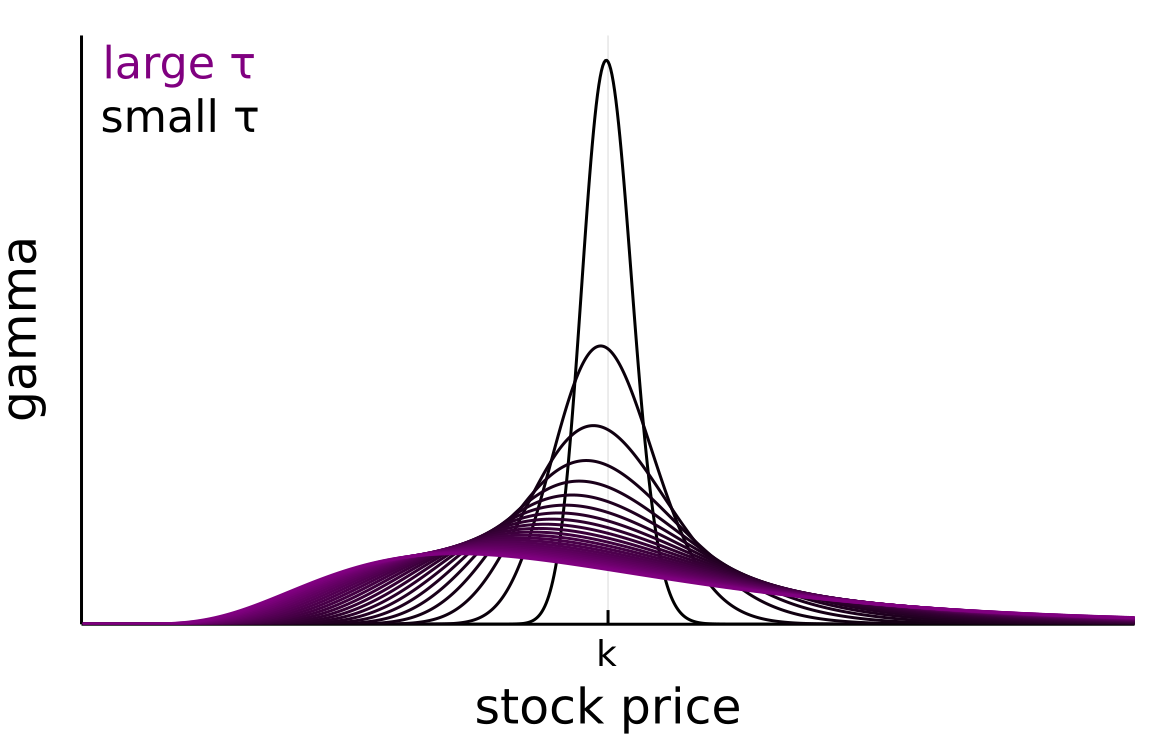
\includegraphics[scale=0.145]{gamma.png}
	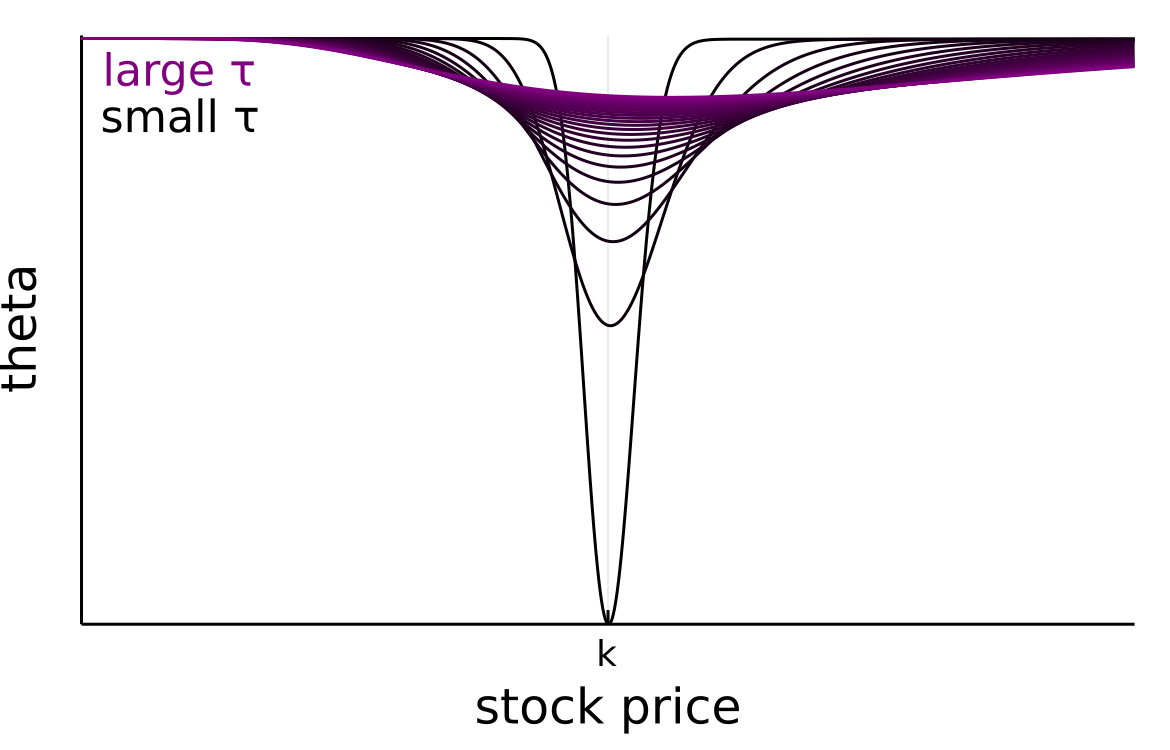
\includegraphics[scale=0.145]{theta.png}
	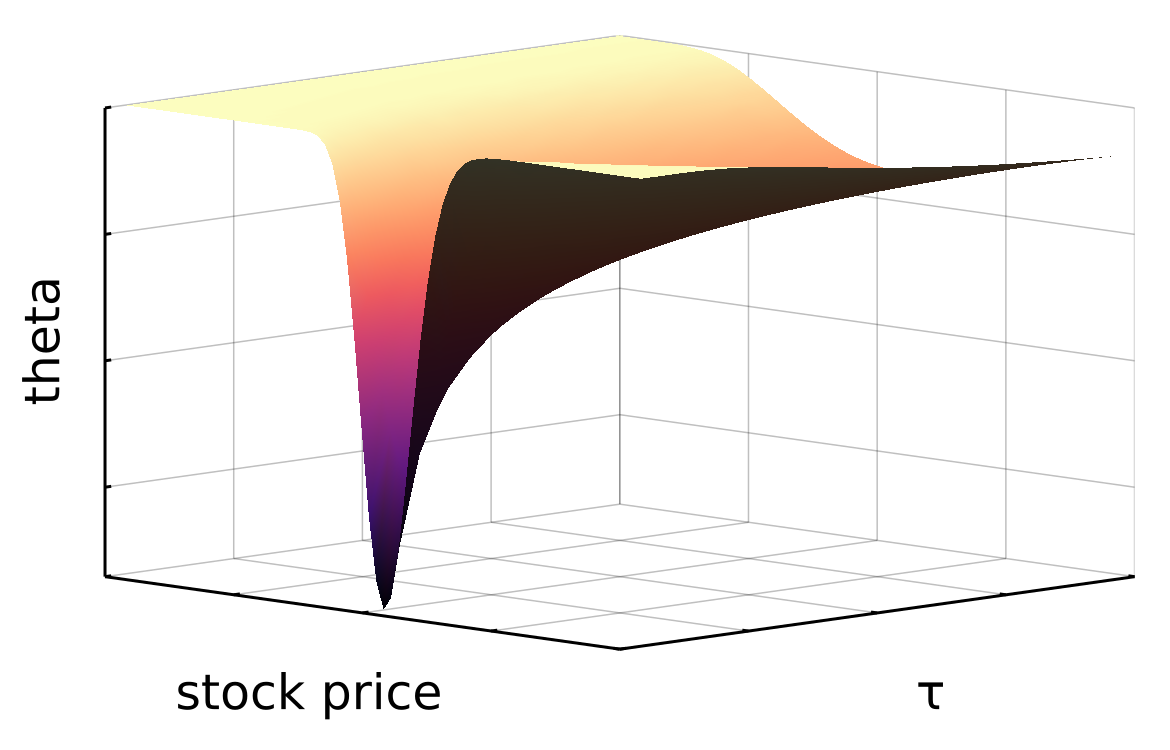
\includegraphics[scale=0.145]{theta_surface.png}
	\caption{The greeks from the Black-Scholes model for a European call. (top-left) delta, (bottom-left) gamma, (top-right) vega, (bottom-right) theta. Also (top-middle) delta vs time, (bottom-middle) premium vs time illustrating theta decay. }
\end{figure*}
	where $d_\pm = \frac{\log(s/k) + (r\pm\sigma^2/2)\tau}{\sigma\sqrt{\tau}}$ and $\Phi$ denotes the standard Gaussian CDF. Note that since $t\in(-\infty, T]$, the time until expiry $\tau$ evolves "backwards" from $\infty$ to 0. As illustrated in Figure 1, this solution converges to the proper boundary conditions. For a put option, the equation is similar except for an overall minus sign and taking $d_\pm \mapsto -d_\pm$:
	
	$$ p_\text{put}(s,\tau) = -s\Phi\left(-d_+\right)  + e^{-r\tau} k \Phi\left(-d_-\right) $$
	
	\strategy{Limitations}
	While extremely useful as a guide for intuition, the Black-Scholes model has some serious limitations in its practical application. Of course the usual assumptions of a perfectly efficient and arbitrage-free market can be challenged, but perhaps the most poignant issues come from assuming lognormal returns with constant volatility $\sigma$ and risk-free rate $r$. Real returns can have distributions with fat tails so by assuming they are lognormal, there is potential to severely underestimate risk. Then of course, the Black-Scholes formula only applies to European options. American options allow for the possibility of early exercise which is not accounted for.
	\\

	\section*{The Greeks}
	
	Options are regularly characterized by a handful of quantities known as \emph{the greeks}. Within the Black-Scholes model, the greeks can be computed explicitly providing an analytic picture of options. But in real markets, for the reasons provided before, these analytic results must be taken with a grain of salt.
	
	\strategy{Delta}
	The first greek, delta, is defined as the option's sensitivity to changes in the underlying price. That is:
	$$ \Delta \equiv \frac{\partial p}{\partial s} $$
	For calls, $\Delta$ is positive while for puts, $\Delta$ is negative. The absolute value of $\Delta$ is always between 0 and 1 since deeply OTM options will be unaffected by movements in the underlying while deeply ITM options will have a value just like having the underlying itself. 
	
	Within the Black-Scholes model, we can calculate an exact expression to find 
	$$\Delta = \Phi(d_+) $$	
	In Figure 2, $\Delta$ is plotted separately against both stock price and time. As we approach expiry, delta approaches a sharp step function $\theta(s-k)$.
	
	\strategy{Theta}
	Theta is defined by how the option price changes as the time to expiration $\tau$ becomes smaller:
	$$ \Theta \equiv - \frac{\partial p}{\partial \tau} $$
	All else equal, an option will always lose value as expiry gets closer since there is less \emph{time value} (i.e. potential for profit). This effect is known as \emph{theta decay} and is illustrated in Figure 2 (bottom-right) where a call premium is plotted against time. The exact Black-Scholes theta is
	$$ \Theta = -\frac{\sigma}{\sqrt{4\tau}} s\phi(d_+) - kre^{-r\tau}\Phi(d_-) $$
	where $\phi$ is the standard Gaussian PDF. Theta is always negative and has its largest magnitude near the strike price.

	\strategy{Vega}
	Vega is defined as the option's sensitivity to volatility in the underlying:
	$$ \mathcal{V}\equiv \frac{\partial p}{\partial \sigma} $$
	Vega is always positive since an increase in volatility implies an increase in probability that an option would end in-the-money. The exact expression from Black-Scholes is found to be
	$$ \mathcal{V} = s\sqrt{\tau}\,\phi(d_1) $$
	It is worth wondering how meaningful this is since the Black-Scholes model assumes constant volatility. Indeed, this only makes sense if we consider the volatility as parameterizing an ensemble of geometric Brownian motion processes. So this is \emph{not} how the option value changes as the volatility changes in time, but rather this is how different option prices might compare at the same $\tau$ but with different underlying volatilities. 
	
	From the plot of vega in Figure 2, it is evident that options are particularly sensitive to volatility when the underlying price is close to strike. Since the option is right ATM, any considerable volatility at all would be enough move it OTM or ITM. Also we can see that when expiry is a long way off, the option value is more sensitive to volatility. This is intuitively true since there is more time for the underlying to make extreme moves, especially with high volatility.
	
	
	\strategy{Gamma}
	Finally, gamma is defined as $\Delta$'s sensitivity to changes in underlying value. In terms of the option price, we have
	$$ \Gamma \equiv \frac{\partial^2 p}{\partial s^2} $$
	Since $\Delta$ is monotonically increasing, $\Gamma$ is always positive. A large value of gamma indicates that the option is becoming \emph{increasingly sensitive} to the underlying's value. It is accelerating. This is a good thing for option owners when the underlying is moving as expected.
	
	The Black-Scholes expression for gamma is
	$$ \Gamma = \frac{\phi(d_+)}{\sigma s \sqrt{\tau}} $$
	\\
	
	\begin{thebibliography}{3}
		\bibitem{haugh}
		\href{http://www.columbia.edu/~mh2078/FoundationsFE/BlackScholes.pdf}{Haugh, 2016, notes for Foundations of Financial Engineering at Columbia - The Black Scholes Model}
		
		\bibitem{chan}
		\href{https://www.math.cuhk.edu.hk/~rchan/teaching/math4210/chap08.pdf}{R. Chan, 2021, notes for Financial Mathematics - Chapter 8 - Black-Scholes Equations}
	\end{thebibliography}
	
	
	
\end{document}